\section{\ExercisePrefixEmbeddedC Touchdisplay ansteuern \optional}
In diesem Abschnitt lernst du die Ansteuerung des 480 * 320 Pixel großen Touchdisplays kennen. Zunächst wirst du den Bildschirm in verschiedene Farben ausfüllen und die dafür benötigte Farbcodierung kennenlernen. Anschließend wirst du Funktionen implementieren, um auf dem Bildschirm regelmäßige Muster und Texte auszugeben. Alle in dieser Aufgabe verwendeten Funktionen müssen in der Datei display.c implementiert werden. 

\begin{table}[]
	\centering
	\caption{Wichtige Funktionen und Variablen für das Display}
	\label{displayInfo}
	\begin{tabular}{|l|l|}
		\hline
		\textbf{Funktionen/Variablen} & \textbf{Beschreibung} \\ \hline
		void drawRect(int16\_t x, int16\_t y, int16\_t w, int16\_t h, uint16\_t color) & Zeichnet die Umrandung eines Rechtecks in der Farbe color mit der Breite w und der Höhe h an die Stelle x,y. \\ \hline
		void fillRect(int x1, int y1, int w, int h, int fillcolor) & Zeichnet ein ausgefülltes Rechteck in der Farbe fillcolor mit der Breite w und der Höhe h an die Stelle x,y. \\ \hline
		void drawPixel(int16\_t x, int16\_t y, uint16\_t color) & Zeichnet ein Pixel an x,y mit der Farbe color. \\ \hline
		void fillScreen(int color) & Füllt den gesamten Bildschirm mit der Farbe color. \\ \hline
		uint16\_t color565(uint8\_t r, uint8\_t g, uint8\_t b) & Umwandlung von RGB in HEX 565. \\ \hline
	\end{tabular}
\end{table}

\subsection{Bildschirm umfärben}
Um den Bildschirm auszufüllen können die in der Library vordefinierten Farben verwendet werden:
\hints{
\item  
BLACK   0x0000
\item 
BLUE    0x001F
\item 
RED     0xF800
\item 
GREEN   0x07E0
\item 
YELLOW  0xFFE0
\item 
WHITE   0xFFFF
}

Das Display verwendet eine 565-Hexadezimal-Codierung für Farben. Bei der 565-Codierung werden 5 Bits für Rot, 6 Bits für Gelb und 5 Bits für Blau verwendet.
Zunächst implementierst du die Funktion color565(uint8\_t r, uint8\_t g, uint8\_t b), um 888-RGB-Farben in 565-RGB-Farben umzuwandeln. Zur Validierung deiner Implementation kannst du folgende 888-RGB-Farben verwenden, und deine 565-Werte mit den vorgegebenen vergleichen.

\begin{table}[]
	\centering
	\caption{RGB-565 Farbwerte}
	\label{rgb565Table}
	\begin{tabular}{|l|l|l|}
		\hline
		\textbf{Farbe} & \textbf{RGB-888} & \textbf{RGB-565} \\ \hline
		Cyan & 0x00EAFF & 0x075F \\ \hline
		Rosa & 0xFC00FF & 0xF81F \\ \hline
		Orange & 0xFFB400 & 0xFDA0 \\ \hline
	\end{tabular}
\end{table}

\begin{figure}
	\begin{centering}
		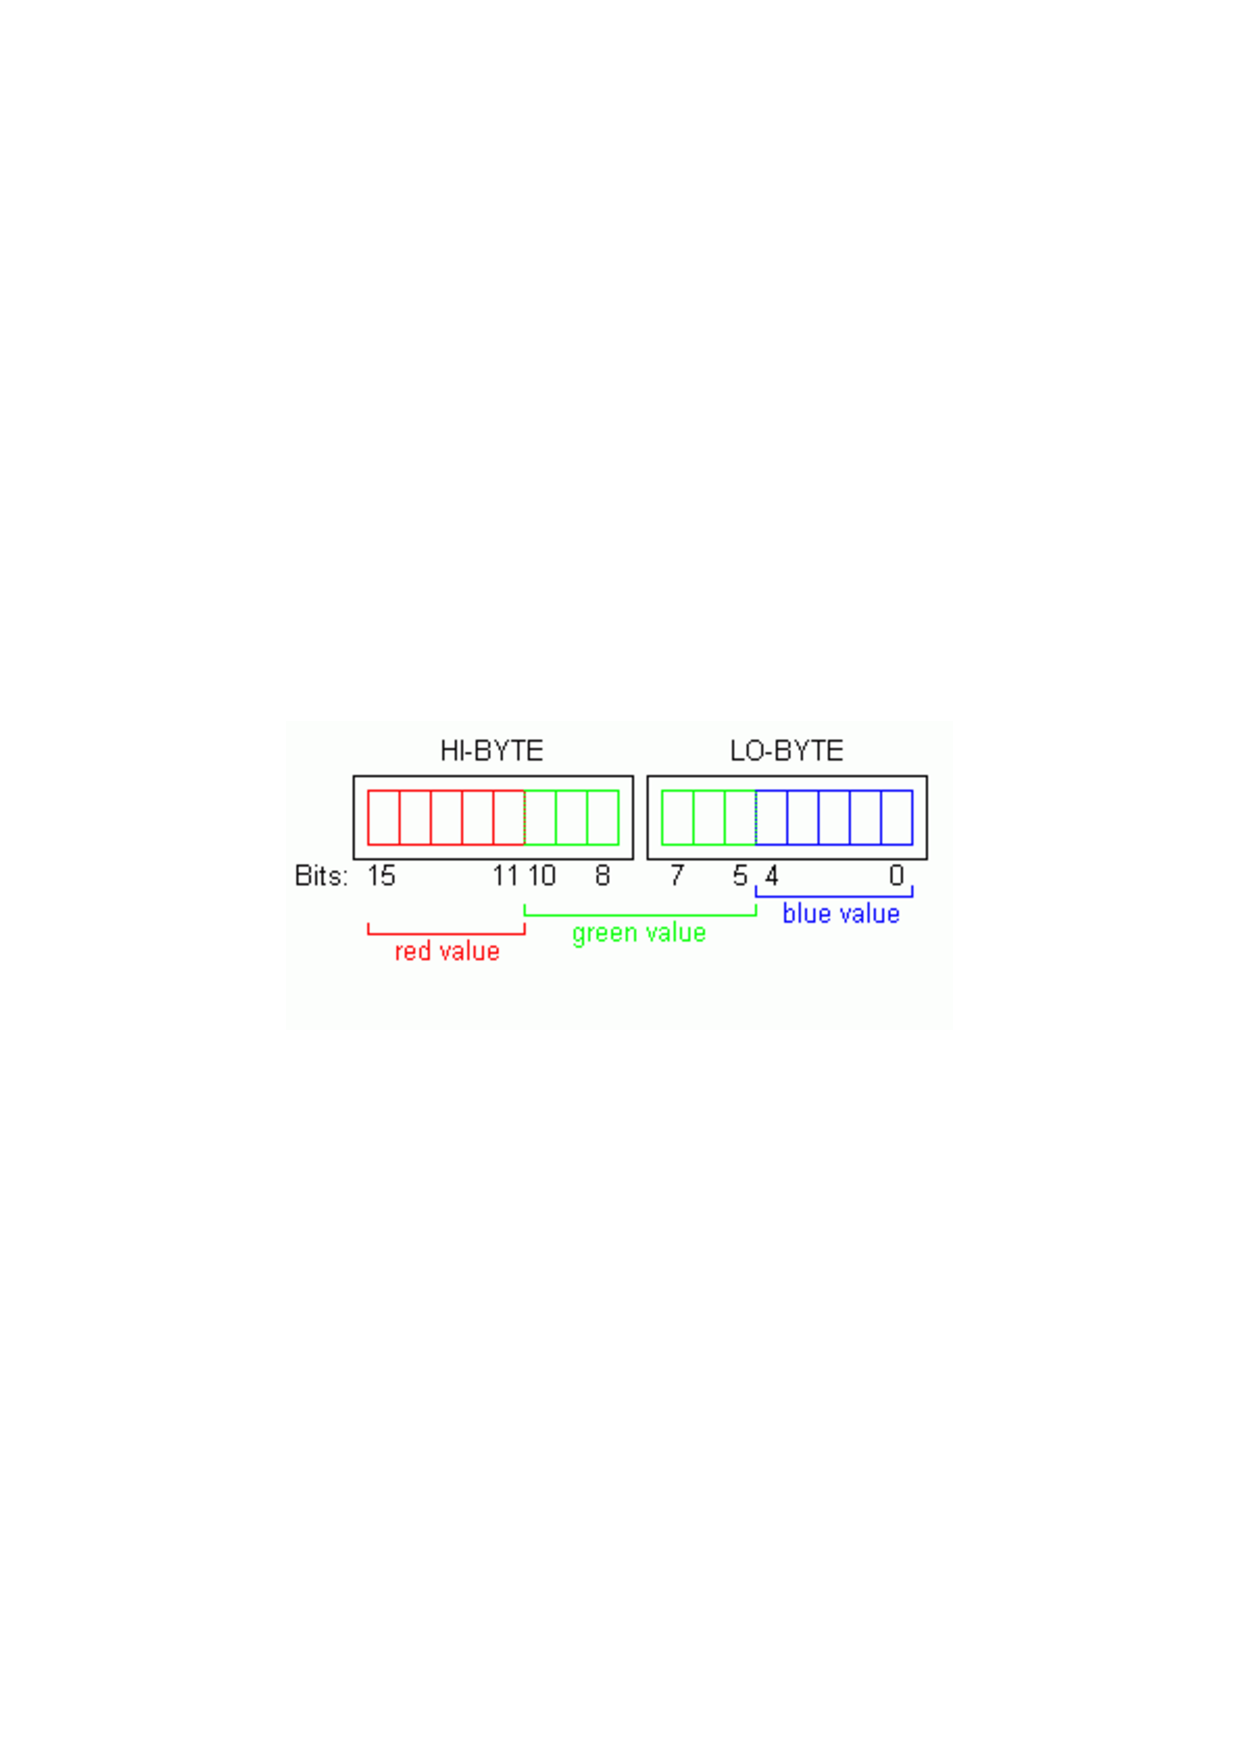
\includegraphics[width=.5\textwidth]{./05_c/figures/rgb565}
		\caption{RGB-565 Codierung}
		\label{fig:rgb565}
	\end{centering}
\end{figure}


\subsection{Regelmäßiges Muster ausgeben}
In diesem Abschnitt implementierst du die Funktion void printPattern(), welche fillRect verwendet um 4 x 4 große Rechtecke im schwarz-weißen Schachbrett-Muster auf dem Display anzuzeigen.
\subsection{Text ausgeben}
\begin{figure}
	\begin{centering}
		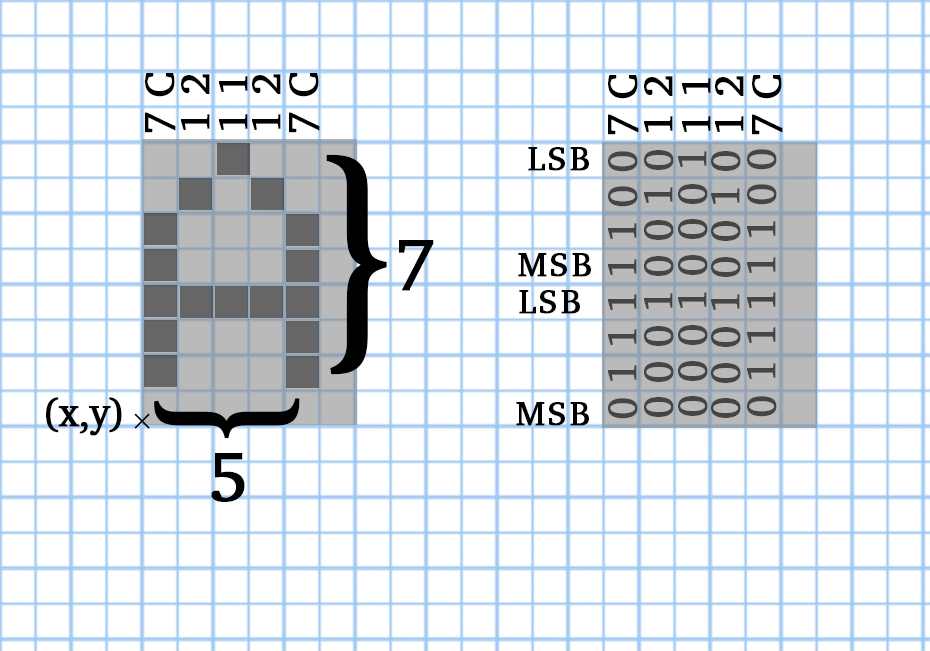
\includegraphics[width=.5\textwidth]{./05_c/figures/ASCII57.png}
		\caption{ASCII 5*7 Schriftart}
		\label{fig:ascii57}
	\end{centering}
\end{figure}
Zum Anzeigen von Buchstaben auf dem Bildschirm wird eine ASCII 5 * 7 Bibliothek verwendet. Diese besteht aus einem Array mit 255 Buchstaben, die jeweils aus f{\"u}nf 8-Bit gro{\ss}en Hexadezimalzahlen bestehen. Die 5 * 7 Bibliothek eignet sich f{\"u}r den 480 * 320 gro{\ss}en Bildschirm, da die Darstellung dier Schriftart mit einer Fl{\"a}che von 35 Pixeln f{\"u}r einen Buchstaben trotzdem sehr gut lesbar ist. Wenn man von einem 1 Pixel Abstand zwischen den Buchstaben ausgeht, passen auf das Display bis zu 3 200 Zeichen. Somit es ist m{\"o}glich l{\"a}ngere Textpassagen auf dem Bildschirm ohne Probleme abzubilden. Die Methode \texttt{drawChar} kann mit Hilfe der ASCII Schriftart Buchstaben an jeder Stelle des Bildschirms in verschiedenen abbilden. Zus{\"a}tzliche Parameter au{\ss}er der Position sind Schriftfarbe, -gr{\"o}{\ss}e und Hintergrundfarbe. Durch die setUp-Methode ist der Bildschirm so eingestellt, dass sich der Koordinatenurpsrung in der unteren linken Ecke des Bildschirms befindet.  

In display.h ist die Schriftart, welche in der Datei glcdfont.h im Array font abgelegt ist, bereits eingebunden. Um globale Grundeinstellungen für die Schriftart festzulegen, wurde bereits die Variablen cursorX, cursorY, textColor, textSize und textBackground deklariert. 

(1.) Implementiere die Set-Funktionen für die Variablen cursorX, cursorY, textColor, textSize und textBackground.

(2.) Die Funktion drawChar soll einen Buchstaben der ASCII-Schriftart auf dem Display an der Position x,y in der Farbe color mit der Hintergrundfarbe bg und der Größe size abbilden. Zunächst muss überprüft werden, ob die angegeben x,y Positionen im gültigen Wertebereich des Display liegen. Sofern die Werte die Grenzen des Bildschirms überschreiten, soll die Funktion drawChar beendet werden. Als nächster Schritt soll auf die richtige Stelle des Array font zugegriffen werden und die Bits der Hexadezimalwerte in Farbwerte intepretiert werden. Abbildung \ref{fig:ascii57} zeigt den Aufbau der Buchstaben im Array font am Beispiel von A. Jeder Buchstabe ist in font an der Position c*5 des Array gespeichert, wenn c für den ASCII-Wert des char steht. Für diesen Buchstaben werden 40 Bits durchiteriert und für jedes Bit, welches gleich 1 ist, wird an dieser Stelle ein Pixel oder Rechteck auf dem Display ausgegeben. Ist die Größe der Schriftart größer als 1, empfiehlt es sich statt drawPixel die Funktion fillRect zu verwenden. 

(3.) Um die Textausgabe auf dem Display für strings zu ermöglichen, müssen weitere Funktionen implementiert werden, die einen automatisierten Cursor verwenden, der die Position des letzten geschriebenen Buchstaben speichert. Die Funktion writeAuto(char c) soll die Aufgabe übernehmen einen Buchstaben c auf dem Display mit hilfe von drawChar zu schreiben und die Position der Cursor cursorX und cursorY zu verändern. Hierbei sind Display-Grenzen und Zeilenumbrüche zu beachten.

(4.) Implementiere die Funktion writeText(char *text), welche einen char Array als Parameter erhält und diesen mithilfe von writeAuto auf dem Display schreiben soll. Außerdem soll noch eine Abwandlung writeTextln(char *text) implementiert werden, welche am Ende des Strings noch einen Zeilenumsprung einfügen soll.

(5.) Zur Ausgabe von Zahlen soll die Funktion writeNumberOnDisplay(uint16\_t *value) implementiert werden, welche Integer in ein char-Array umwandelt und diesen mithilfe von writeText auf dem Display ausgibt. Die Funktion itoa aus der stdlib.h kann zur Lösung dieser Aufgabe hilfreich sein.
